CSP Anlagen beziehen ihre primäre Energiequelle aus der Direct Normal Irradiance (DNI), welche im besten Fall in einem rechten Winkel zu einer Oberfläche ausgerichtet ist, die in der Lage ist die Sonnenstrahlung aufzunehmen. Dieses Potential ist im sogenannten "`sun belt"' am größten. Der "`sun belt"' bezeichnet den Bereich der Erde nördlich und südlich vom zwanzigsten bis zum vierzigsten Breitengrad. Zum jetzigen Zeitpunkt wurden vier Haupttechnologien entwickelt und getestet\cite{viebahn2011}:

\begin{figure}[H]
	\centering
	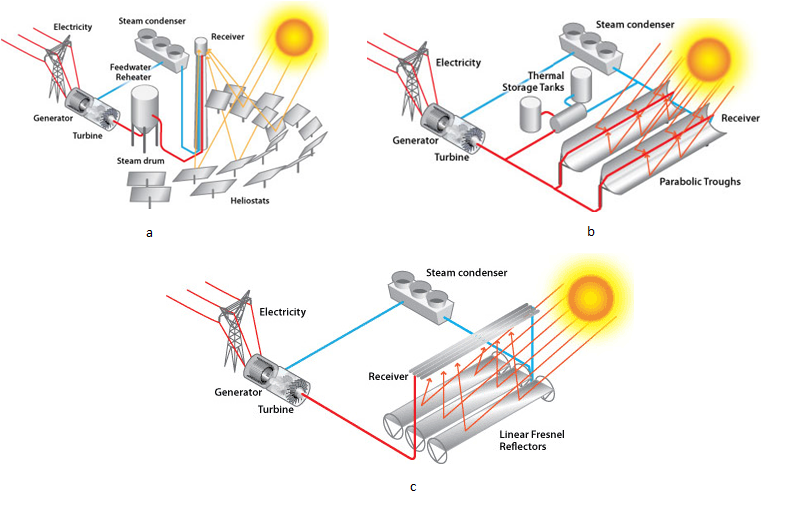
\includegraphics[width=0.9\textwidth,trim=1 1 1 1,clip]{technik.png}
	\caption{CSP Technologien.\ a: Parabolrinnenkraftwerke, b: Solarturmkraftwerke, c: Fresnelrinnenkraftwerke. Quelle:~energy.gov}
	\label{fig:technik}
\end{figure}

\textbf{Parabolrinnenkraftwerke}
\newline
Ein Parabolrinnenkraftwerk besteht aus einer Reihe von parabelförmigen Sonnenkollektoren und einer Gasturbine zur Erzeugung von elektrischer Energie. Zur Überführung der Wärmeenergie von den Kollektoren zur Turbine wird eine Transferflüssigkeit verwendet. Diese besteht meistens aus einem synthetisch hergestellten Öl, welches durch die Kollektoren fließt. Das Öl wird im Anschluss zur Erzeugung von heißem Dampf genutzt, was schlussendlich durch die Turbine strömt. Für die Zukunft werden neue Technologien im Bereich der Transferflüssigkeit angestrebt. So sind Lösungen ohne den Gebrauch von Öl erstrebenswert, da die Verwendung von Öl mit hohen Kosten in der Aufbereitung und Entsorgung verbunden ist. Auch ist die Verwendung von geschmolzenem Sand in der Entwicklung, welches gegenüber Öl eine höhere Effizienz erzielt, da weitaus höhere Temperaturen erreicht werden können.
\cite{viebahn2008}

\textbf{Fresnelrinnenkraftwerke} 
\newline
Im Gegensatz zu Parabolrinnenkraftwerke setzen Fresnelrinnenkraftwerke auf ebene Kollektoren, die im Gegensatz zur Parabolkollektoren die Sonnenstrahlung auf nur einer Achse aufnehmen. Dies hat eine Effizienzminderung zu Folge, da nicht alle Bereiche des Kollektors orthogonal zur Strahlenrichtung ausgerichtet sind. Die Idee der Fresnel Technologie besteht darin, dass durch die Vereinfachte Technik und die dadurch geringeren Kosten den Verlust der Energie kompensieren.
\cite{viebahn2008}

\textbf{Solarturmkraftwerke}
\newline
Solarturmkraftwerke bestehen aus einem Feld von  Kollektoren, die leicht geneigt die Sonnenstrahlung auf einen in der Mitte des Feldes befindlichen Turm reflektieren. Im Turm werden die gebündelten Strahlen dazu genutzt um wieder eine Transferflüssigkeit zu erhitzen, welche zur Erzeugung von Dampf genutzt wird. Ein Vorteil bei diesem Ansatz gegenüber oben Genannten, ist der geringe Transportweg der Energie bis zu Erzeugung von elektrischer Energie. Die Turbine befindet sich meistens direkt im Turm selbst, sodass keine langen Transportwege nötig sind.
\cite{viebahn2008}

\begin{figure}[H]
	\centering
	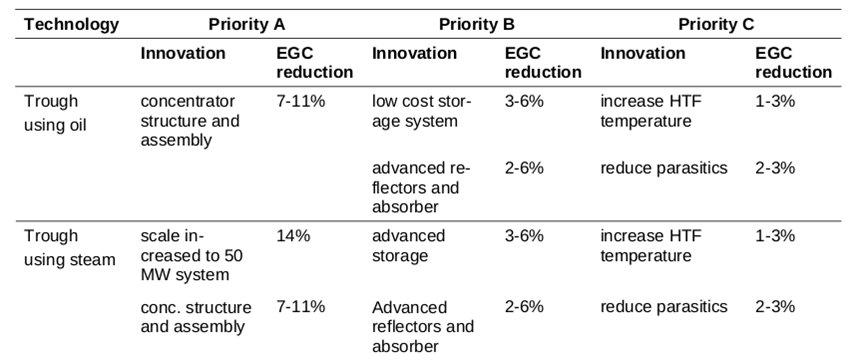
\includegraphics[width=0.9\textwidth,trim=1 1 1 1,clip]{technische_entwicklung1.png}
	\caption{Transferflüssigkeit-Entwicklung~(\cite{viebahn2011})}
	\label{fig:technik_e1}
\end{figure}

Allgemein sind technische Entwicklungen für die Zukunft vor allem in den Bereichen Reflektoren, Speicher, Skalierbarkeit und Temperatur anzusehen~\ref{fig:technik_e1}.
\newline
Reflektoren können in Bezug auf Widerstandsfähigkeit, Reflektionsgrad, Wirkungsgrad, Gewicht und Zusammenbau weiter optimiert werden. Desweitern besteht Innovationspotential für neue Transferflüssigkeiten, die zum Transport der Wärme nötig sind.

\begin{figure}[H]
	\centering
	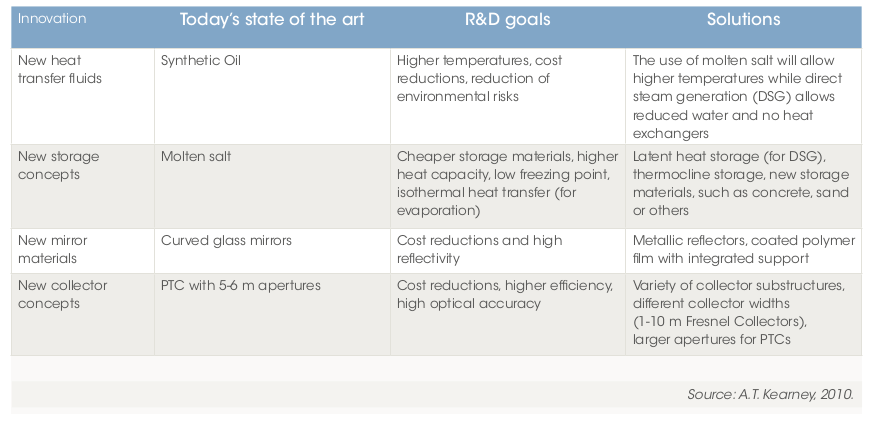
\includegraphics[width=0.9\textwidth,trim=1 1 1 1,clip]{technische_entwicklung2.png}
	\caption{Speicherentwicklung~(\cite{irena2012})}
	\label{fig:technik_e2}
\end{figure}

Um die gewonnene Energie zwischen zu speichern sind moderne Speichertechniken gefragt. Hier gibt es ebenfalls neue Konzepte, die mit geschmolzenem Sand arbeiten um eine höhere Wärmekapazität als herkömmliche Speichermedien zu gewährleisten~\ref{fig:technik_e2}.


